%-------------------------------------------------------------------------
% Design Project Input/Output Module Description
%-------------------------------------------------------------------------

\clearpage
\section{LED Matrix Output Module}
\label{sec-output-ledmatrix}

This output module enables your IoT device to control a 16x24 LED matrix
which can display useful messages and graphics on its large screen; for
example, the matrix can display digital clocks, thermometers, counters
and meters, instrumentation readouts, industrial control indicators,
etc. You can also chain multiples of these displays together! The panel
works using a special HT1632C chip on the back which does most of the
necessary work to display messages for you. Communication with the
matrix happens through a 3-pin serial interface which is easy to work
with.

A sample circuit and Arduino code is shown below to get you started.
The LED matrix has a gray ribbon connector that has a "red strip" on one
side of it. When connecting wires to the connector, the red wire for
power will be on the same side as the "red strip" on the ribbon
connector. The example code will draw a blinking rectangle on the
screen. After setting up the circuit and programming the Arduino, check
that the shape appears on the screen correctly. You can now experiment
with drawing moving shapes or even scrolling text!

\vspace{0.1in}
\begin{minipage}[t]{0.49\tw}
  \vspace{0.0in}
  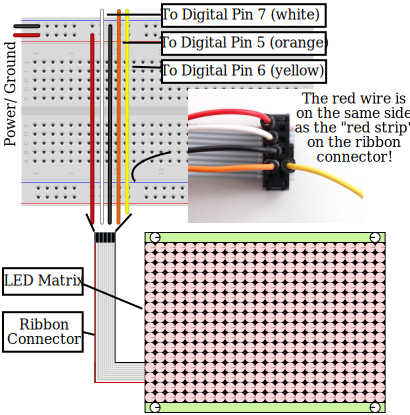
\includegraphics[width=\tw]{output-ledmatrix-annotated.svg.pdf}

\end{minipage}
\hspace{0.1in}
\begin{minipage}[t]{0.49\tw}
  \vspace{0.0in}
  \begin{Verbatim}[gobble=3,fontsize=\small]
    #include "HT1632.h"

    int pin_data = 5; // orange wire
    int pin_wr   = 6; // yellow wire
    int pin_cs   = 7; // white wire

    HT1632LEDMatrix matrix =
      HT1632LEDMatrix(pin_data, pin_wr, pin_cs);

    void setup() {
      Serial.begin(9600);
      matrix.begin(HT1632_COMMON_16NMOS);
      matrix.fillScreen();
      delay(500);
    }
  \end{Verbatim}

  \BF{RECTANGLES}:
  \vspace{0.1in}

  Use drawRect( x\_coordinate, y\_coordinate, rect\_width, rect\_height,
  value ). In this example, we draw a rectangle at point (6, 4), that
  is half the width and half the height of the entire matrix. Then we
  clear it. Use "fillRect" to draw a filled rectangle.

  \begin{Verbatim}[gobble=3,fontsize=\small]
    void loop() {
      matrix.drawRect(6, 4,
                matrix.width()/2,
                matrix.height()/2, 1);
      matrix.writeScreen();
      delay(500);
      matrix.clearScreen();
      delay(500);
    }

  \end{Verbatim}

\end{minipage}
\newpage
\begin{minipage}[t]{0.45\tw}
  \vspace{0.0in}

  \BF{PIXELS}:
  \vspace{0.1in}

  Use drawPixel( x\_coord, y\_coord, value ). In this example, we draw a
  pixel at (0, 0), delay \wu{500}{ms}, clear the pixel, and wait another
  \wu{500}{ms}.

  \begin{Verbatim}[gobble=3,fontsize=\small]
    void loop() {
      matrix.drawPixel(0, 0, 1);
      matrix.writeScreen();
      delay(500);
      matrix.drawPixel(0, 0, 0);
      delay(500);
    }
  \end{Verbatim}

  \BF{LINES}:
  \vspace{0.1in}

  Use drawLine( x1\_coord, y1\_coord, x2\_coord, y2\_coord, value ). In this
example, we draw an X and then clear it.

  \begin{Verbatim}[gobble=3,fontsize=\small]
    void loop() {
      matrix.drawLine(0, 0,
                matrix.width()-1,
                matrix.height()-1, 1);
      matrix.drawLine(matrix.width()-1, 0,
                0, matrix.height()-1, 1);
      matrix.writeScreen();
      delay(500);
      matrix.clearScreen();
      delay(500);
    }
  \end{Verbatim}
\end{minipage}
\hspace{0.3in}
\begin{minipage}[t]{0.49\tw}
  \vspace{0.0in}

  \BF{CIRCLES}:
  \vspace{0.1in}

  Use \IT{drawCircle( x\_coord, y\_coord, radius, value )}. The coordinates are
for the center of the circle. In this example we draw a circle and clear it.
Use "fillCircle" to draw a filled circle instead.

  \begin{Verbatim}[gobble=3,fontsize=\small]
    void loop() {
      matrix.drawCircle(
                matrix.width()/2-1, matrix.height()/2-1,
                8, 1);
      matrix.writeScreen();
      delay(500);
      matrix.clearScreen();
      delay(500);
    }
  \end{Verbatim}

  \BF{TEXT}:
  \vspace{0.1in}

  Use:
  \begin{Verbatim}[gobble=3,fontsize=\small]
    - matrix.setCursor(x\_coord, y\_coord)
    - matrix.print( text\_to\_print )
  \end{Verbatim}

  In this example, we draw two lines of text!

  \begin{Verbatim}[gobble=3,fontsize=\small]

    void loop() {
      matrix.setTextSize(1);  // size 1 == 8 pixels high
      matrix.setTextColor(1); // 'lit' LEDs

      matrix.setCursor(0, 0); // start at top left
      matrix.print("Curi");
      matrix.setCursor(0, 8); // next line, 8 pixels down
      matrix.print("e'14");
      matrix.writeScreen();
      delay(500);
      matrix.clearScreen();
      delay(500);
    }
  \end{Verbatim}
\end{minipage}

%Questions:
